\documentclass{beamer}
%
% Choose how your presentation looks.
%
% For more themes, color themes and font themes, see:
% http://deic.uab.es/~iblanes/beamer_gallery/index_by_theme.html
%
\mode<presentation>
{
  \usetheme{NYU}      % or try Darmstadt, Madrid, Warsaw, ...
  \usecolortheme{default} % or try albatross, beaver, crane, ...
  \usefonttheme{default}  % or try serif, structurebold, ...
  \setbeamertemplate{navigation symbols}{}
  \setbeamertemplate{caption}[numbered]
} 

\usepackage[english]{babel}
\usepackage[T1]{fontenc}
\usepackage[utf8x]{inputenc}
\usepackage{hyperref}
\begin{document}
\title[EE2227]{Control System}
\author{EE18BTECH11024\\K,Yaswanth Naidu}
\institute{IITH}
\date{\today}
\titlegraphic{\hfill
\includegraphics[height=1.5cm]{nyu_shanghai}}



\begin{frame}
  \titlepage
\end{frame}
\item \textbf{Question 4}
\item \textbf{  For a unity feedback control system with the forward path transfer function
    $${G(s)} = \frac{k}{s(s+2)}$$
\\The peak resonant magnitude $M_{r}$ of the closed loop frequency is 2.The corresponding value of the gain K is
 }
\item \textbf{solution}
\\Given:
\\ For a unity feedback control system ${G(s)} = \frac{k}{s(s+2)}$ and resonant peak $M_{r}$=2
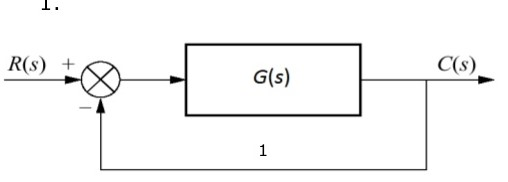
\includegraphics[width=.6\textwidth]{yeswanth (2).jpg}
\\we can find its closed loop transfer function as,
\begin{equation}
    C(s)=[R(S)-H(S)C(S)]G(S)=R(S)G(S)-H(S)C(S)G(S)
\end{equation}
\begin{equation}
    C(S)+H(S)C(S)G(S)=R(S)G(S)
\end{equation}
\begin{equation}
    C(S)[1+G(S)H(S)]=R(S)G(S
\end{equation}
\begin{equation}
    \dfrac{C(s)}{R(s)}=T(s)=\dfrac{G(s)}{1+G(s)H(s)}=\dfrac{\dfrac{K}{s(s+2)}}{1+\dfrac{K}{s(s+2)*1}}=\dfrac{K}{s^2+2s+K}
\end{equation}
\\standard equation of$T(s)$=\dfrac{\omega_{n}^2}{s^2+2S\xi^\omega_{n}+\omega_{n}^2}
\\formula for resonant peak as $M_{r}$=\dfrac{1}{2\xi(1-(\xi)^2)^\dfrac{1}{2}}
\\given resonant peak  $M_{r}$=2
\begin{equation}
    \dfrac{DC Gain}{2\xi(1-(\xi)^2)^\dfrac{1}{2}}=2
    \\here DC gain is 1
\end{equation}
\\squaring on both sides
\\16\xi^2(\xi^2-1)=1
\\$putting$ \xi^2=x
\\ \begin{equation}
    16x^2-16x+1=0
\end{equation}
\begin{equation}
    x=\xi^2=\dfrac{2-\sqrt{3}}{4}
\end{equation}
\begin{equation}
    x=\xi^2=\dfrac{2+\sqrt{3}}{4}
\end{equation}
\\ characteristic equation is $$s^2+2s+k$$
\\comparing it with standard equation we get $\omega_{n}$^2=k
\\2\xi^$\omega_{n}$=2
\\$$\xi=\dfrac{1}{\omega_{n}}=\dfrac{1}{k^\dfrac{1}{2}}$$
\\$$k=\dfrac{1}{\xi^2}=\dfrac{4}{2-\sqrt{3}} = 14.92$$

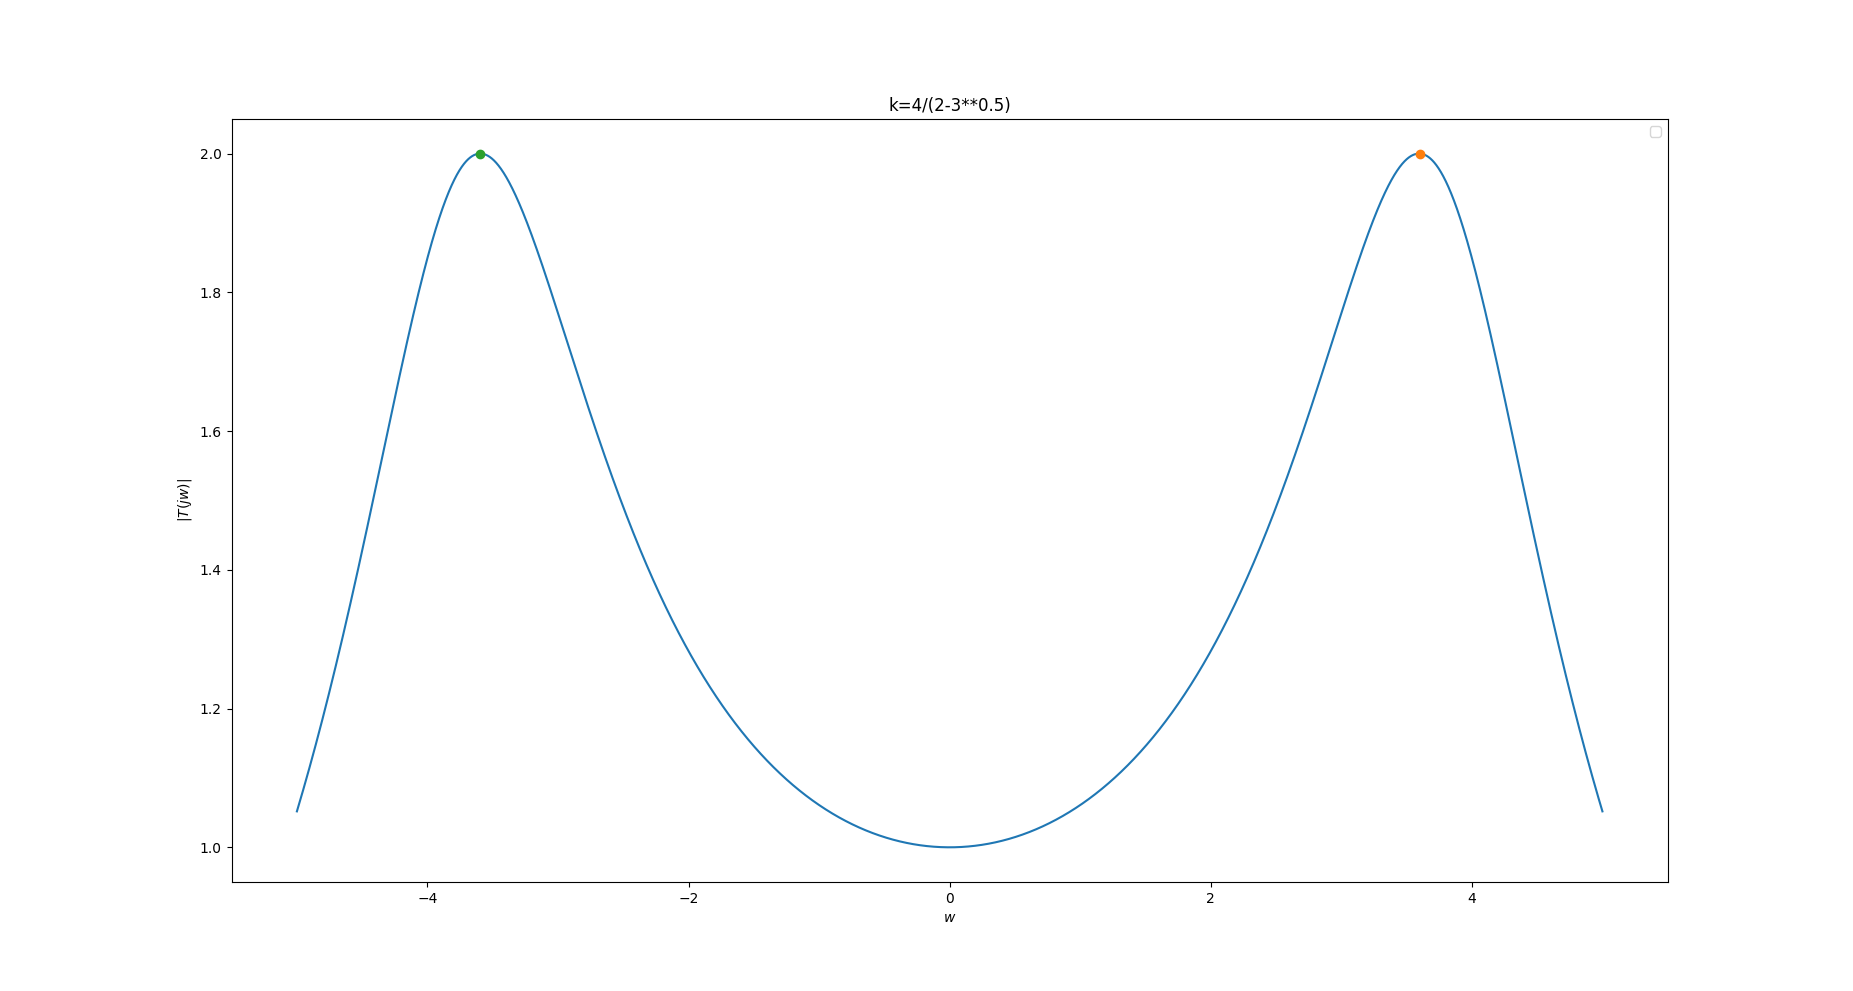
\includegraphics[width=1.2\textwidth]{gate_plot1.png}
\end{document}


